% !TEX root = ../paper.tex
\section{Interaction techniques} \label{sec:techniques}
In this section we will illustrate and describe the interaction techniques we developed in order to exchange data between mobile phones and large displays.
This is done so that we are capable of comparing them to one another in an empirical way.

There were several criteria behind the choice of these techniques. 
The main one was that users would be able to walk up to a large display and utilize them, which means that they should be as intuitive and natural as possible. 
\cref{tab:techniqueCriteria} shows the set of criteria that we based our choices of techniques on.

\begin{table}[H]
	\centering
	\begin{tabular}{|p{0.2\columnwidth}|p{0.7\columnwidth}|}
		\hline
		\rowcolor[HTML]{9B9B9B} 
		\textbf{Criteria} & \textbf{Description} \\ \hline
		Natural feel & There must be a natural and intuitive feel to the techniques in some way. \\ \hline
		Number of hands & There must be both one-handed and two-handed techniques. \\ \hline
		Previously used & To avoid designing and testing a set of novel techniques, we had the criterion that all techniques must have been used by others before we would use them. \\ \hline
		Complexity & The techniques must differ in their complexity and therefore we included techniques with different amount of steps. \\ \hline
		Activation method & The way each technique is activated must be different from each other. \\ \hline
	\end{tabular}
	\label{tab:techniqueCriteria}
\end{table}
%Two-handed techniques which are techniques that require both hands.


All technique themes were found in the literature.
We then created a mirror version of each technique so they each would have a \push and \pull version.
\push means that the user will be pushing information from the mobile to the large display, and \pull means the oposite, the user will pull information from the screen onto the mobile device. 

Eight techniques were chosen in the end: \alltechniques, each with a \push and \pull variant

The \grab technique \cref{fig:grabTechnique} is used in \todo{add reference} by Ikemasu et al. as part of an system for exchanging information between different devices. Benko and Wilson \todo{add reference} used the \grab technique in a system were the user would interact with visualizations inside a dome. \grab is a combination of two aforementioned techniques and the pointing technique used by Scheible et al. in \todo{add reference}.
This technique was chosen because we wanted to simulate the feeling of picking up an object of interest and placing it on a desired location.
\grab is a complex technique, requiring a series of steps as well as using both hands to complete the interaction.
The \push version of this technique is completed as follows: the user first grab a object of interest from the telephone by pinching it with his fingers \cref{fig:grabTechniqueA}, closing his hand, and metaphorically putting the object in his hands.
The user then raises his closed hand and aims at the screen where he wants to place the object \cref{fig:grabTechniqueB}.
The final step is to open the hand over the desired placement of the object on the large display \cref{fig:grabTechniqueC}.
The \pull version is a bit different.
The user first places his open hand over the object of interest on the large display \cref{fig:grabTechniqueC}.
The user then closes hand over the object \cref{fig:grabTechniqueB} and finally places it on his phone by touching it with his closed hand \cref{fig:grabTechniqueA}.  

\begin{figure}[H]
	\subfloat[]{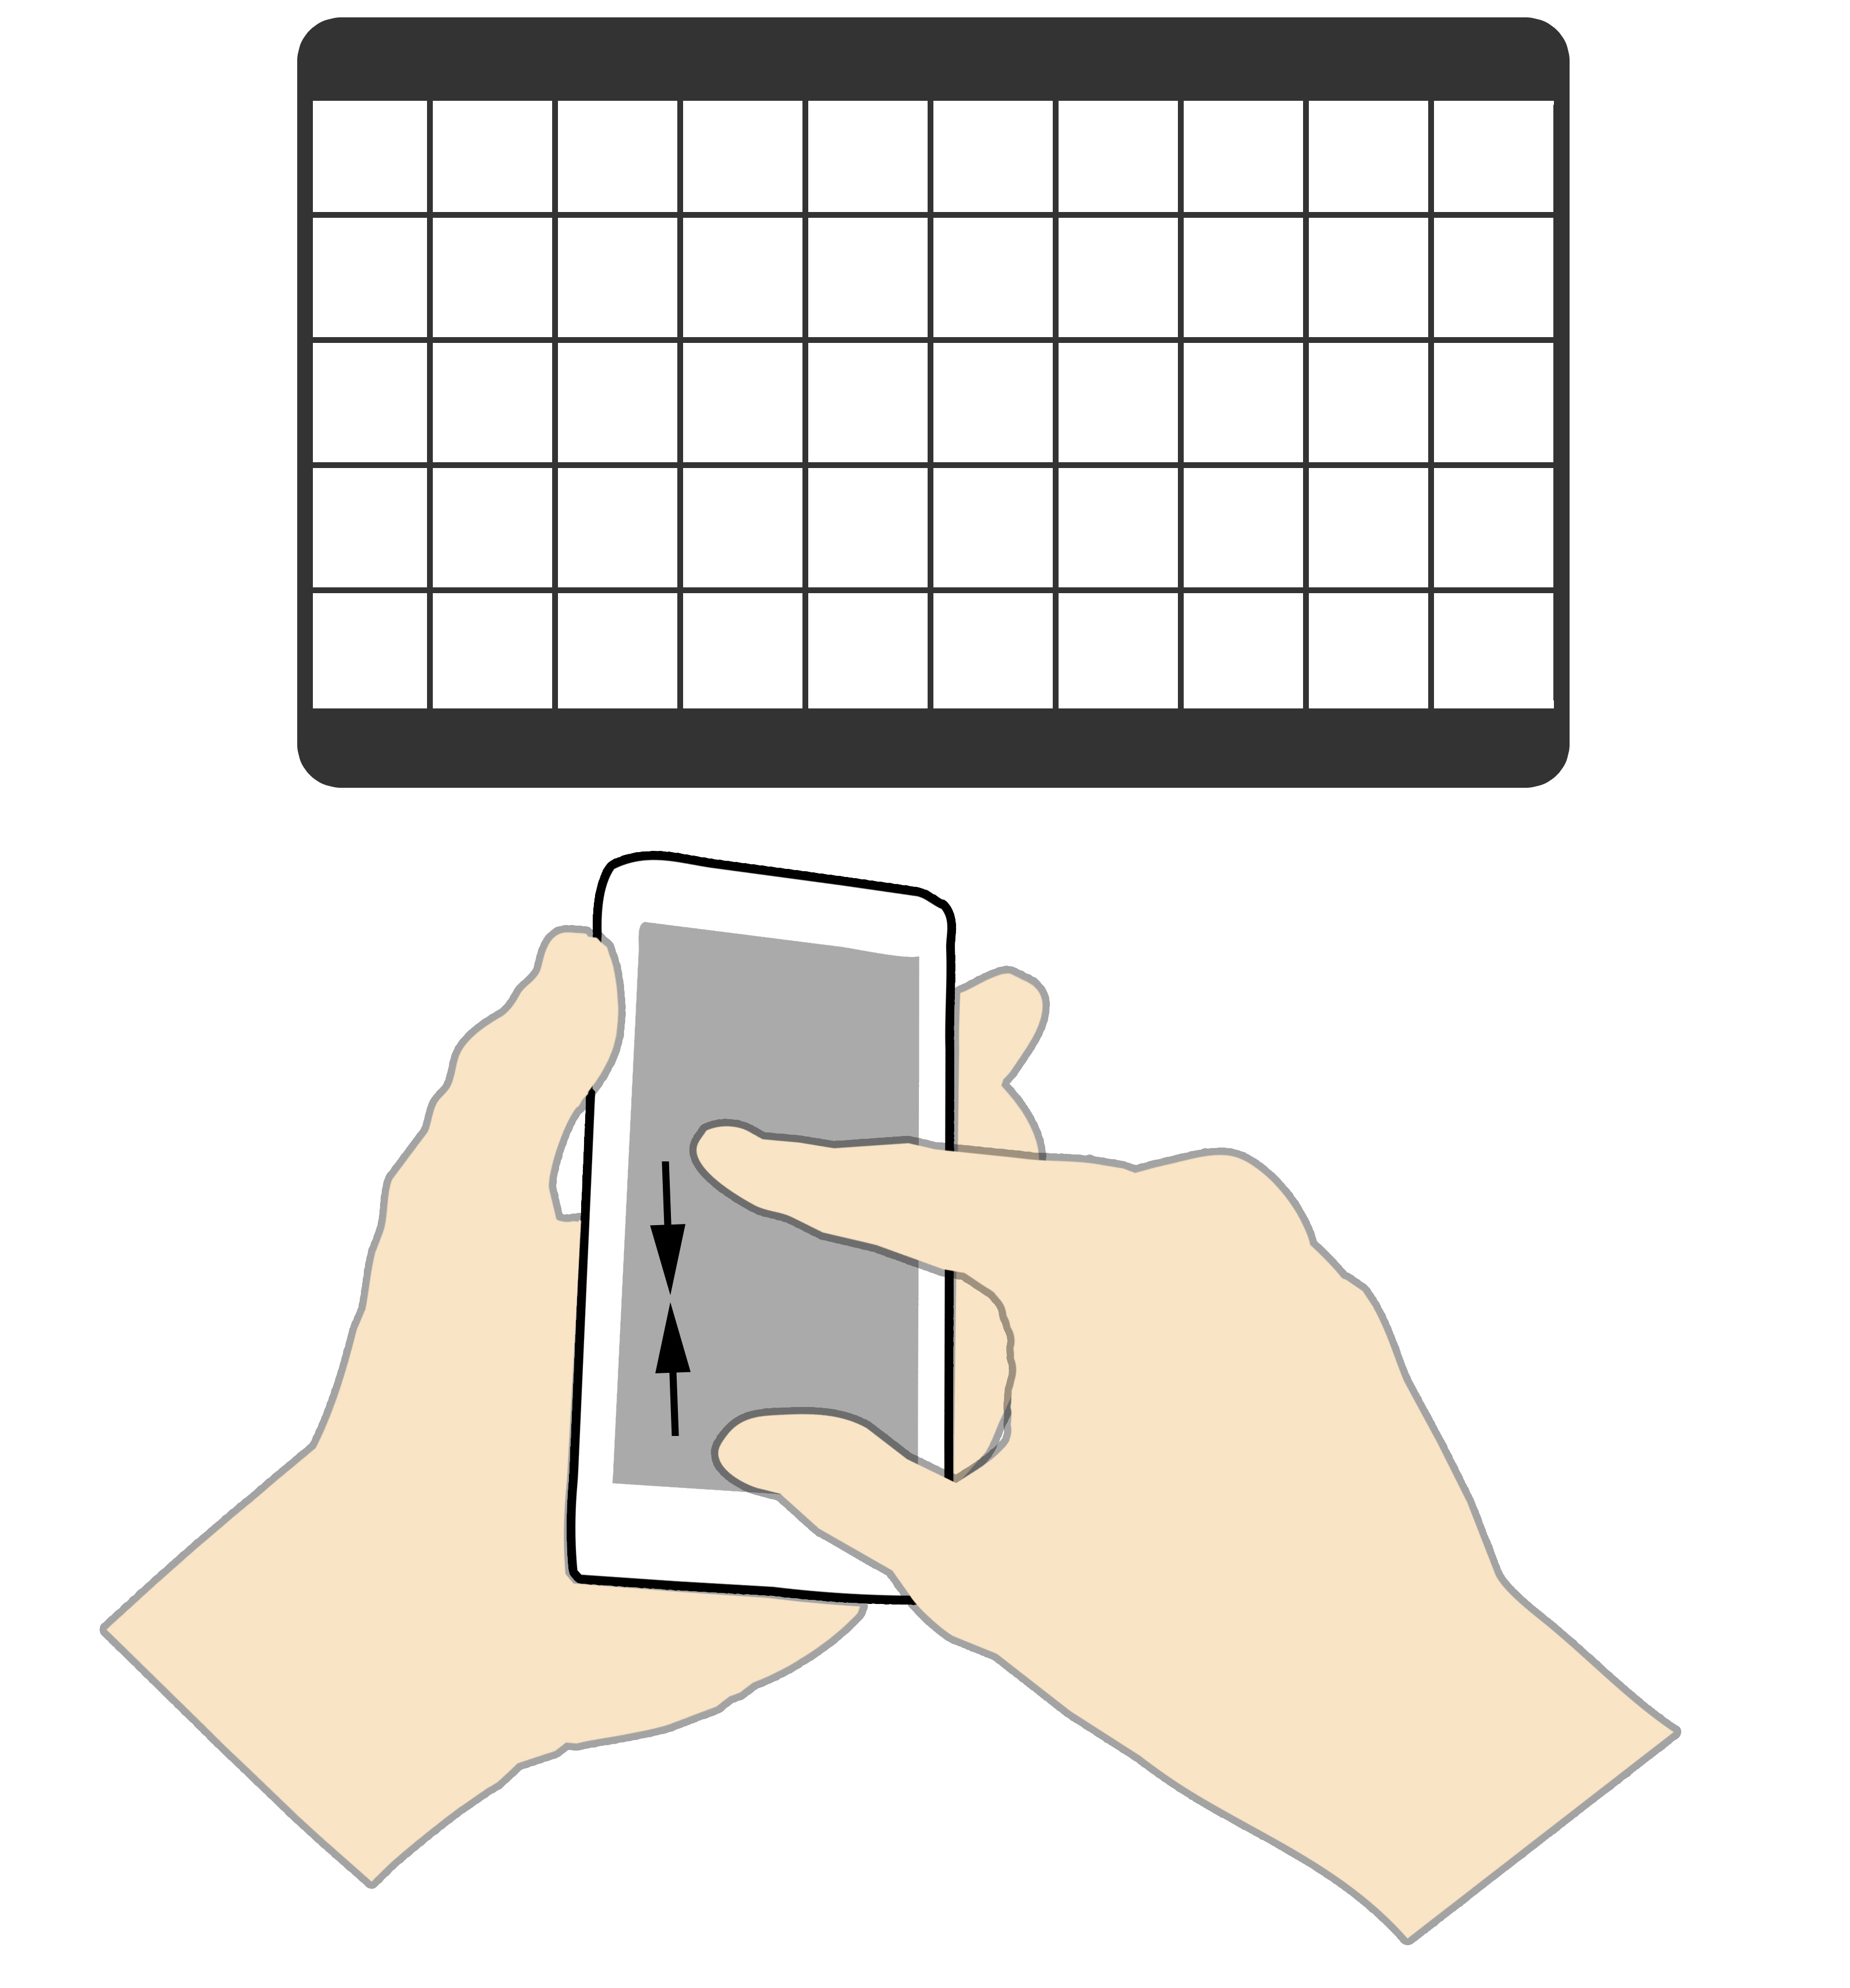
\includegraphics[width = 0.33\columnwidth]{images/grab_a.jpg}\label{fig:grabTechniqueA}}
	\subfloat[]{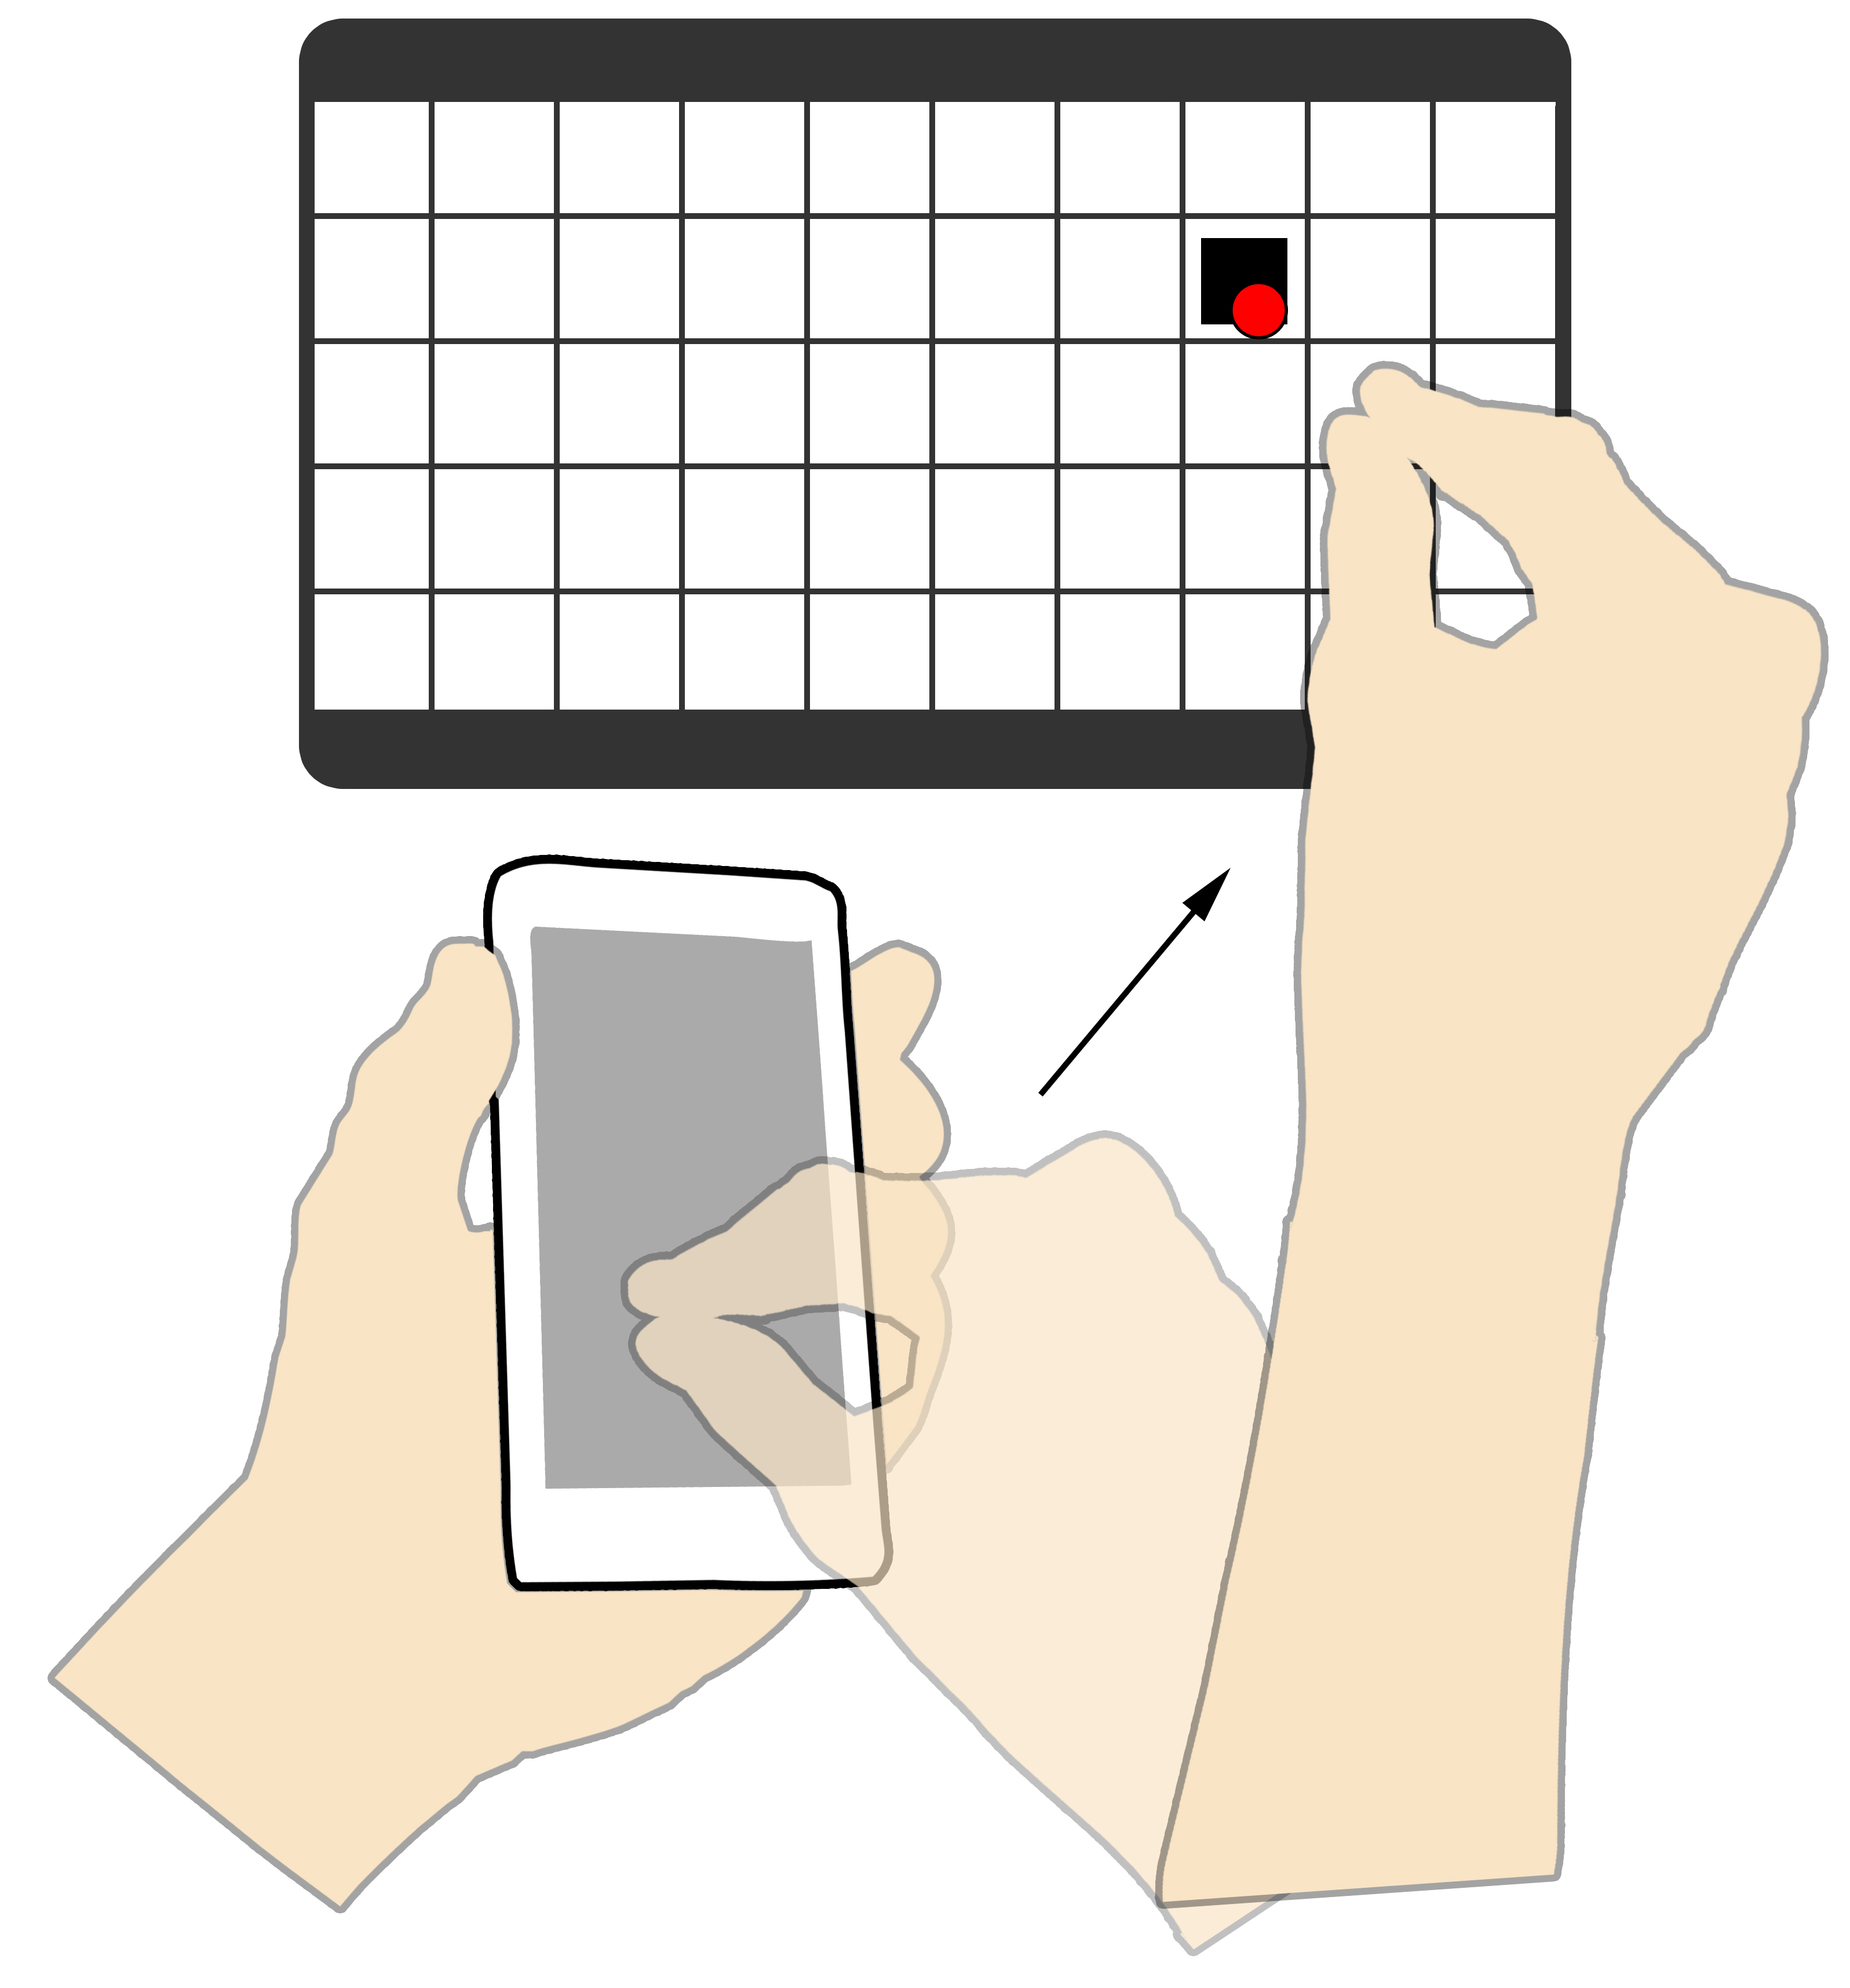
\includegraphics[width = 0.33\columnwidth]{images/grab_b.jpg}\label{fig:grabTechniqueB}}
	\subfloat[]{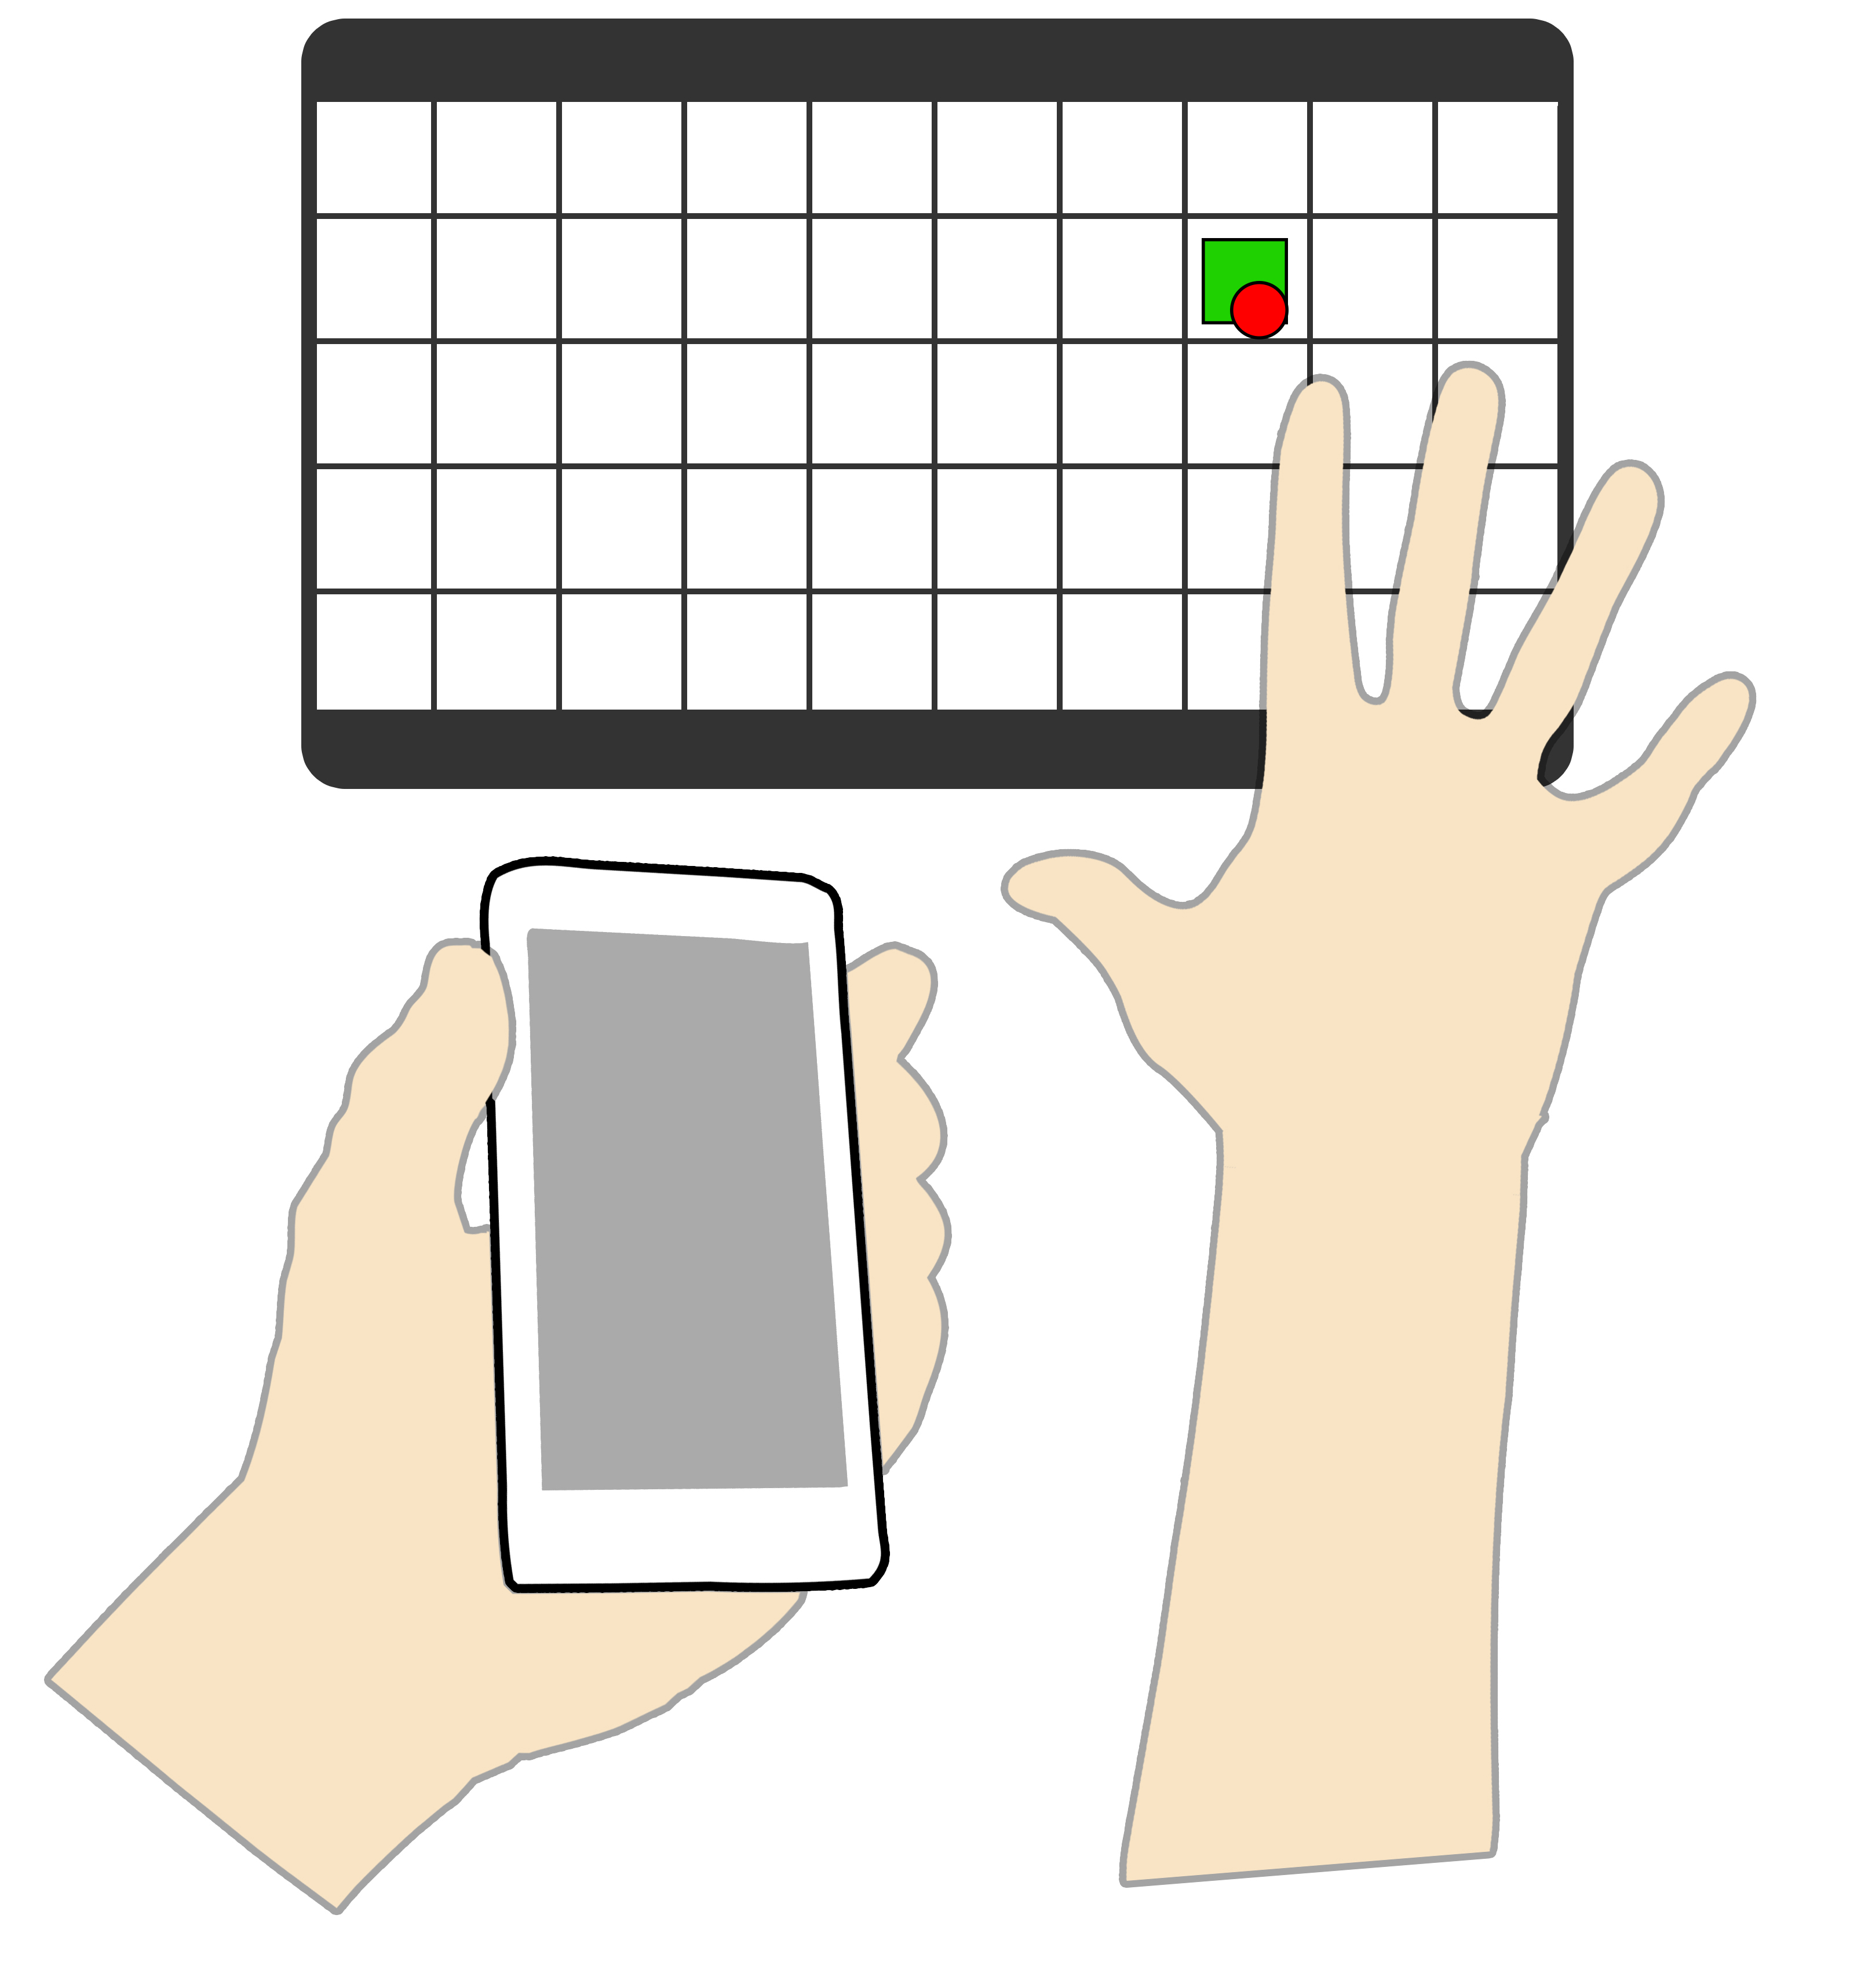
\includegraphics[width = 0.33\columnwidth]{images/grab_c.jpg}\label{fig:grabTechniqueC}}
	\label{fig:grabTechnique}
\end{figure}

The \swipe technique \cref{fig:swipeTechnique} was utilized by Bragdon et. al \todo{add ref} in Code Space.
He developed a system that would support developer meetings with the help of smart phones and the Kinect. Bragdon describes the technique as \emph{``cross-device interaction with touch and air pointing''} and the swiping motion is described as \emph{``flicking up on the touch screen''}.
This technique was chosen because it has a very simplistic design, with a very low level of complexity since it requires very few steps to activate.
It is also a one handed technique and requires very little effort from the user to use.
The \push and \pull version of this technique are very similar.
First the user points at the desired location with the phone in a stretched arm \cref{fig:swipeTechniqueA} and then swipes his finger on the screen \cref{fig:swipeTechniqueC}.
The direction he swipes depends on whether he wants to \push or \pull information.
If he swipes away from himself, he pushes information to the screen.
If he swipes towards himself, he is pulling information from the screen onto the device.  

\begin{figure}[H]
	\subfloat[]{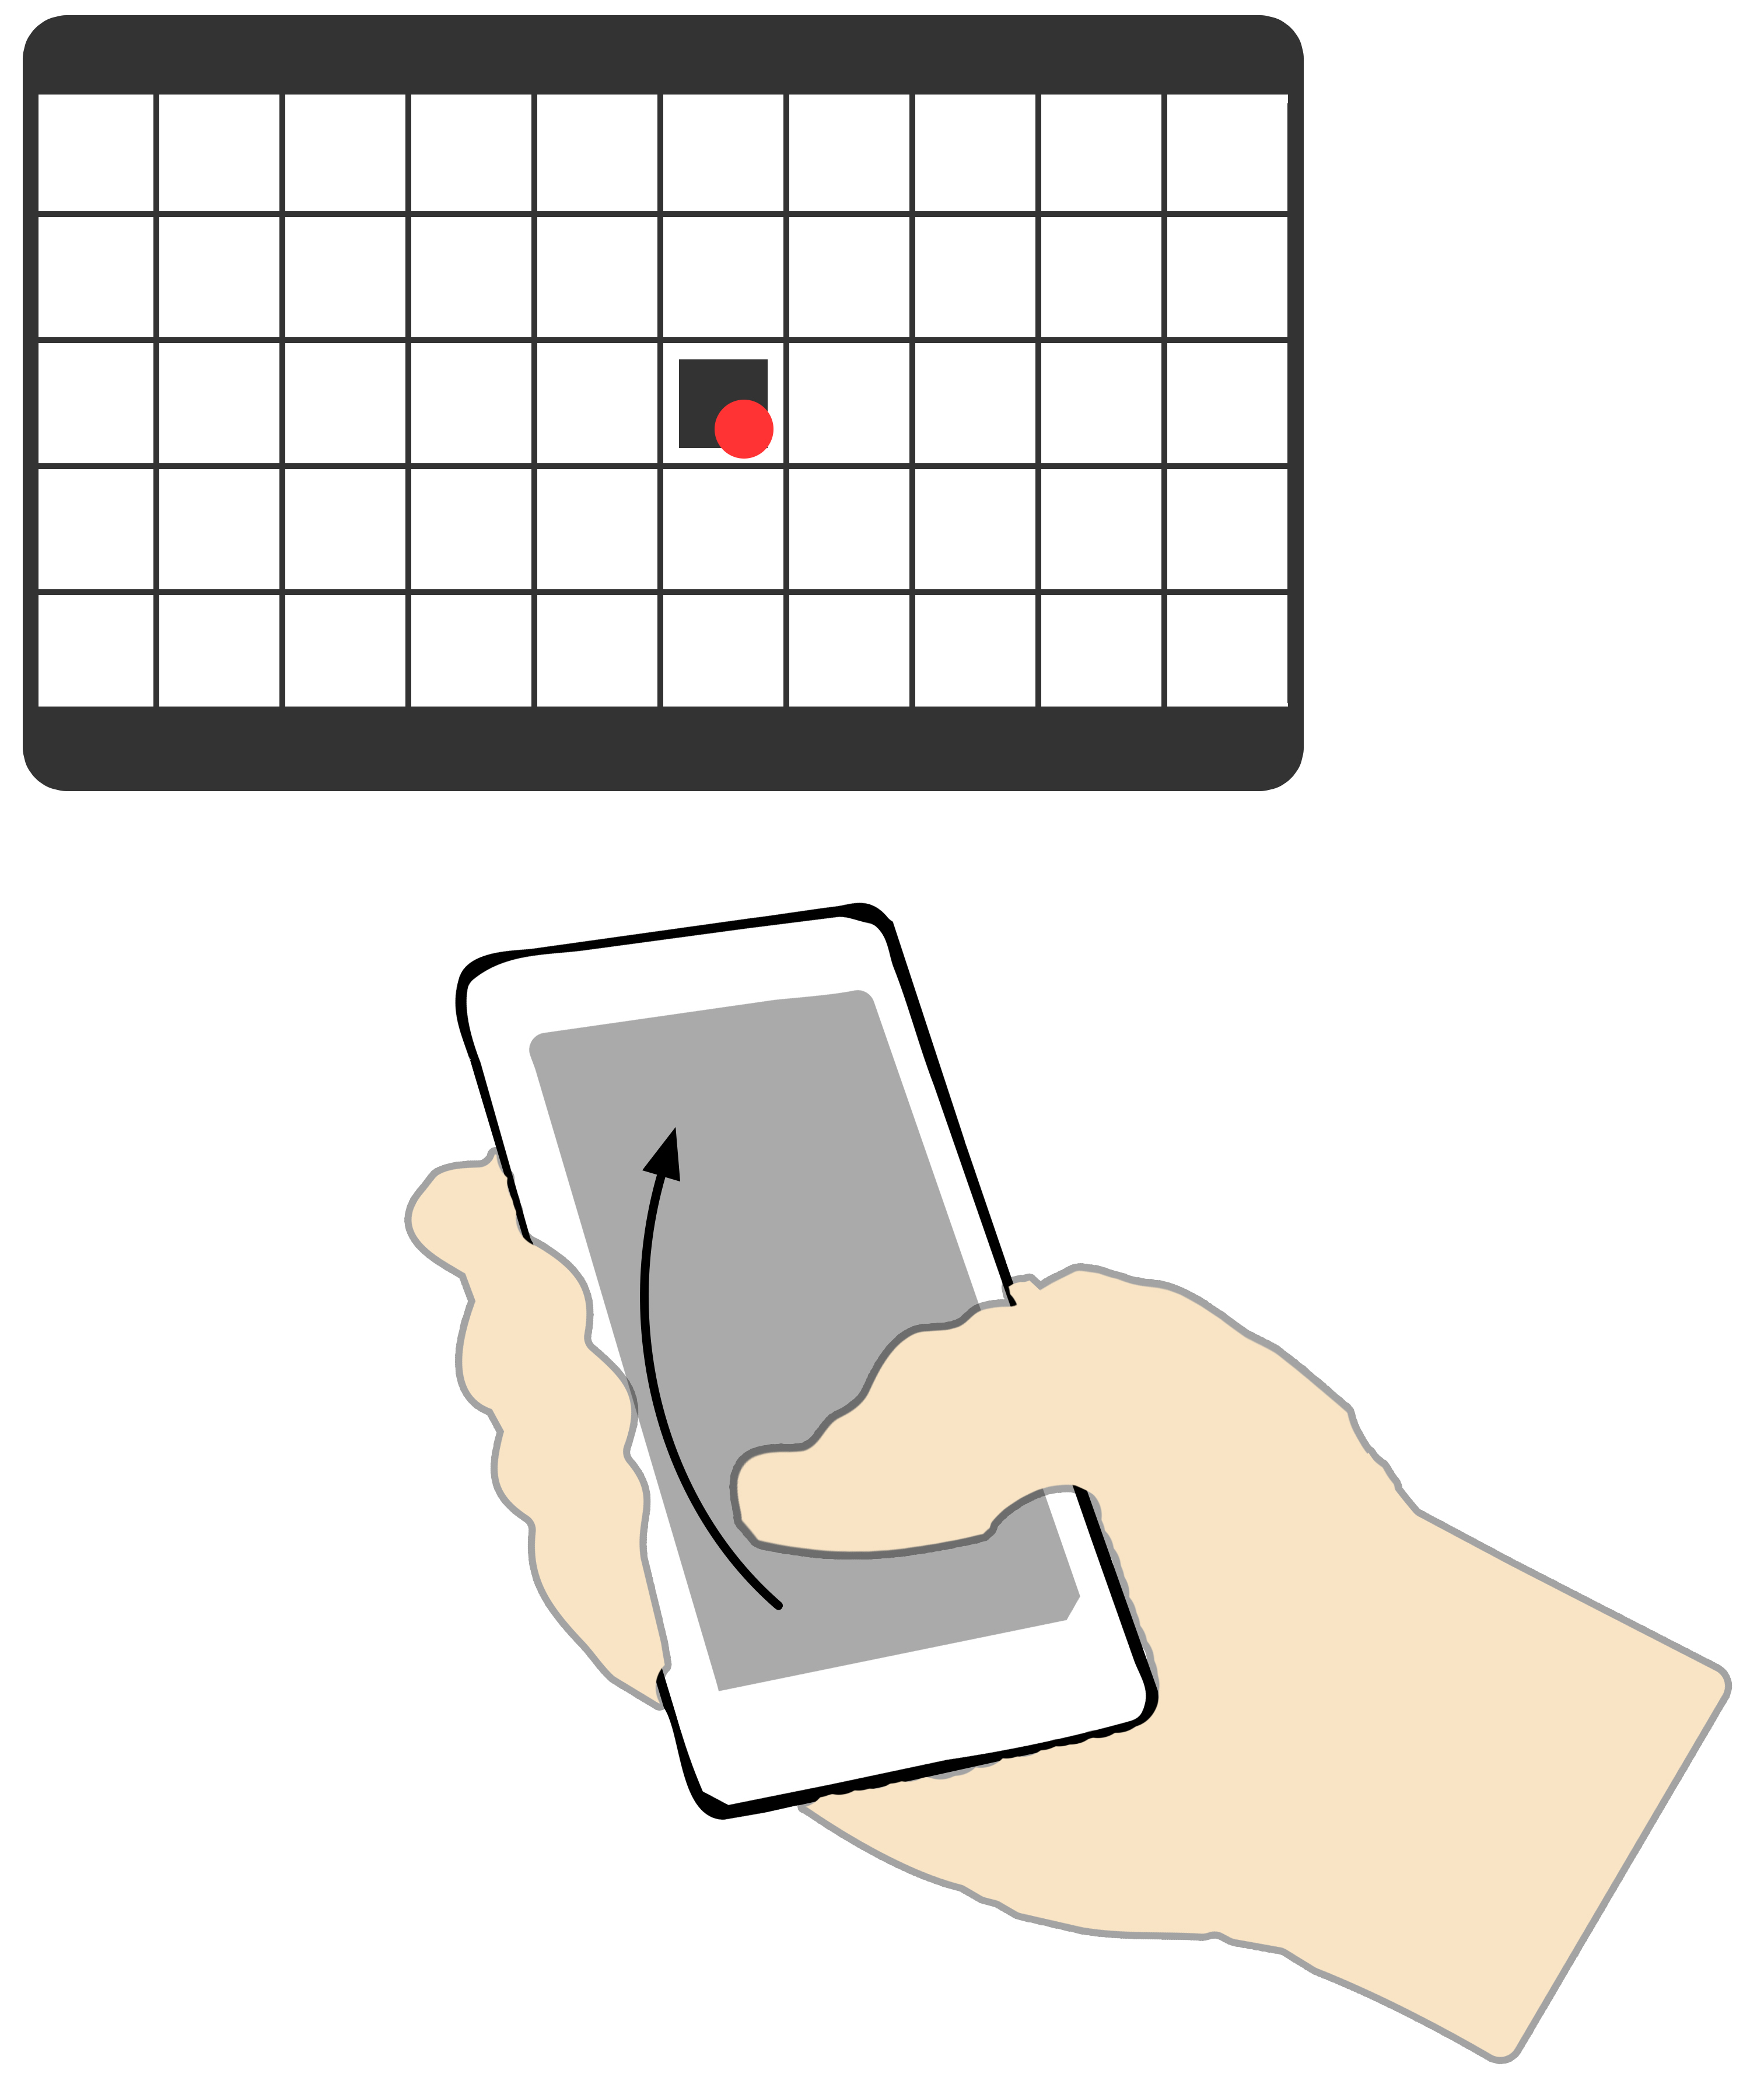
\includegraphics[width = 0.33\columnwidth]{images/swipe_a.jpg}\label{fig:swipeTechniqueA}}
	\subfloat[]{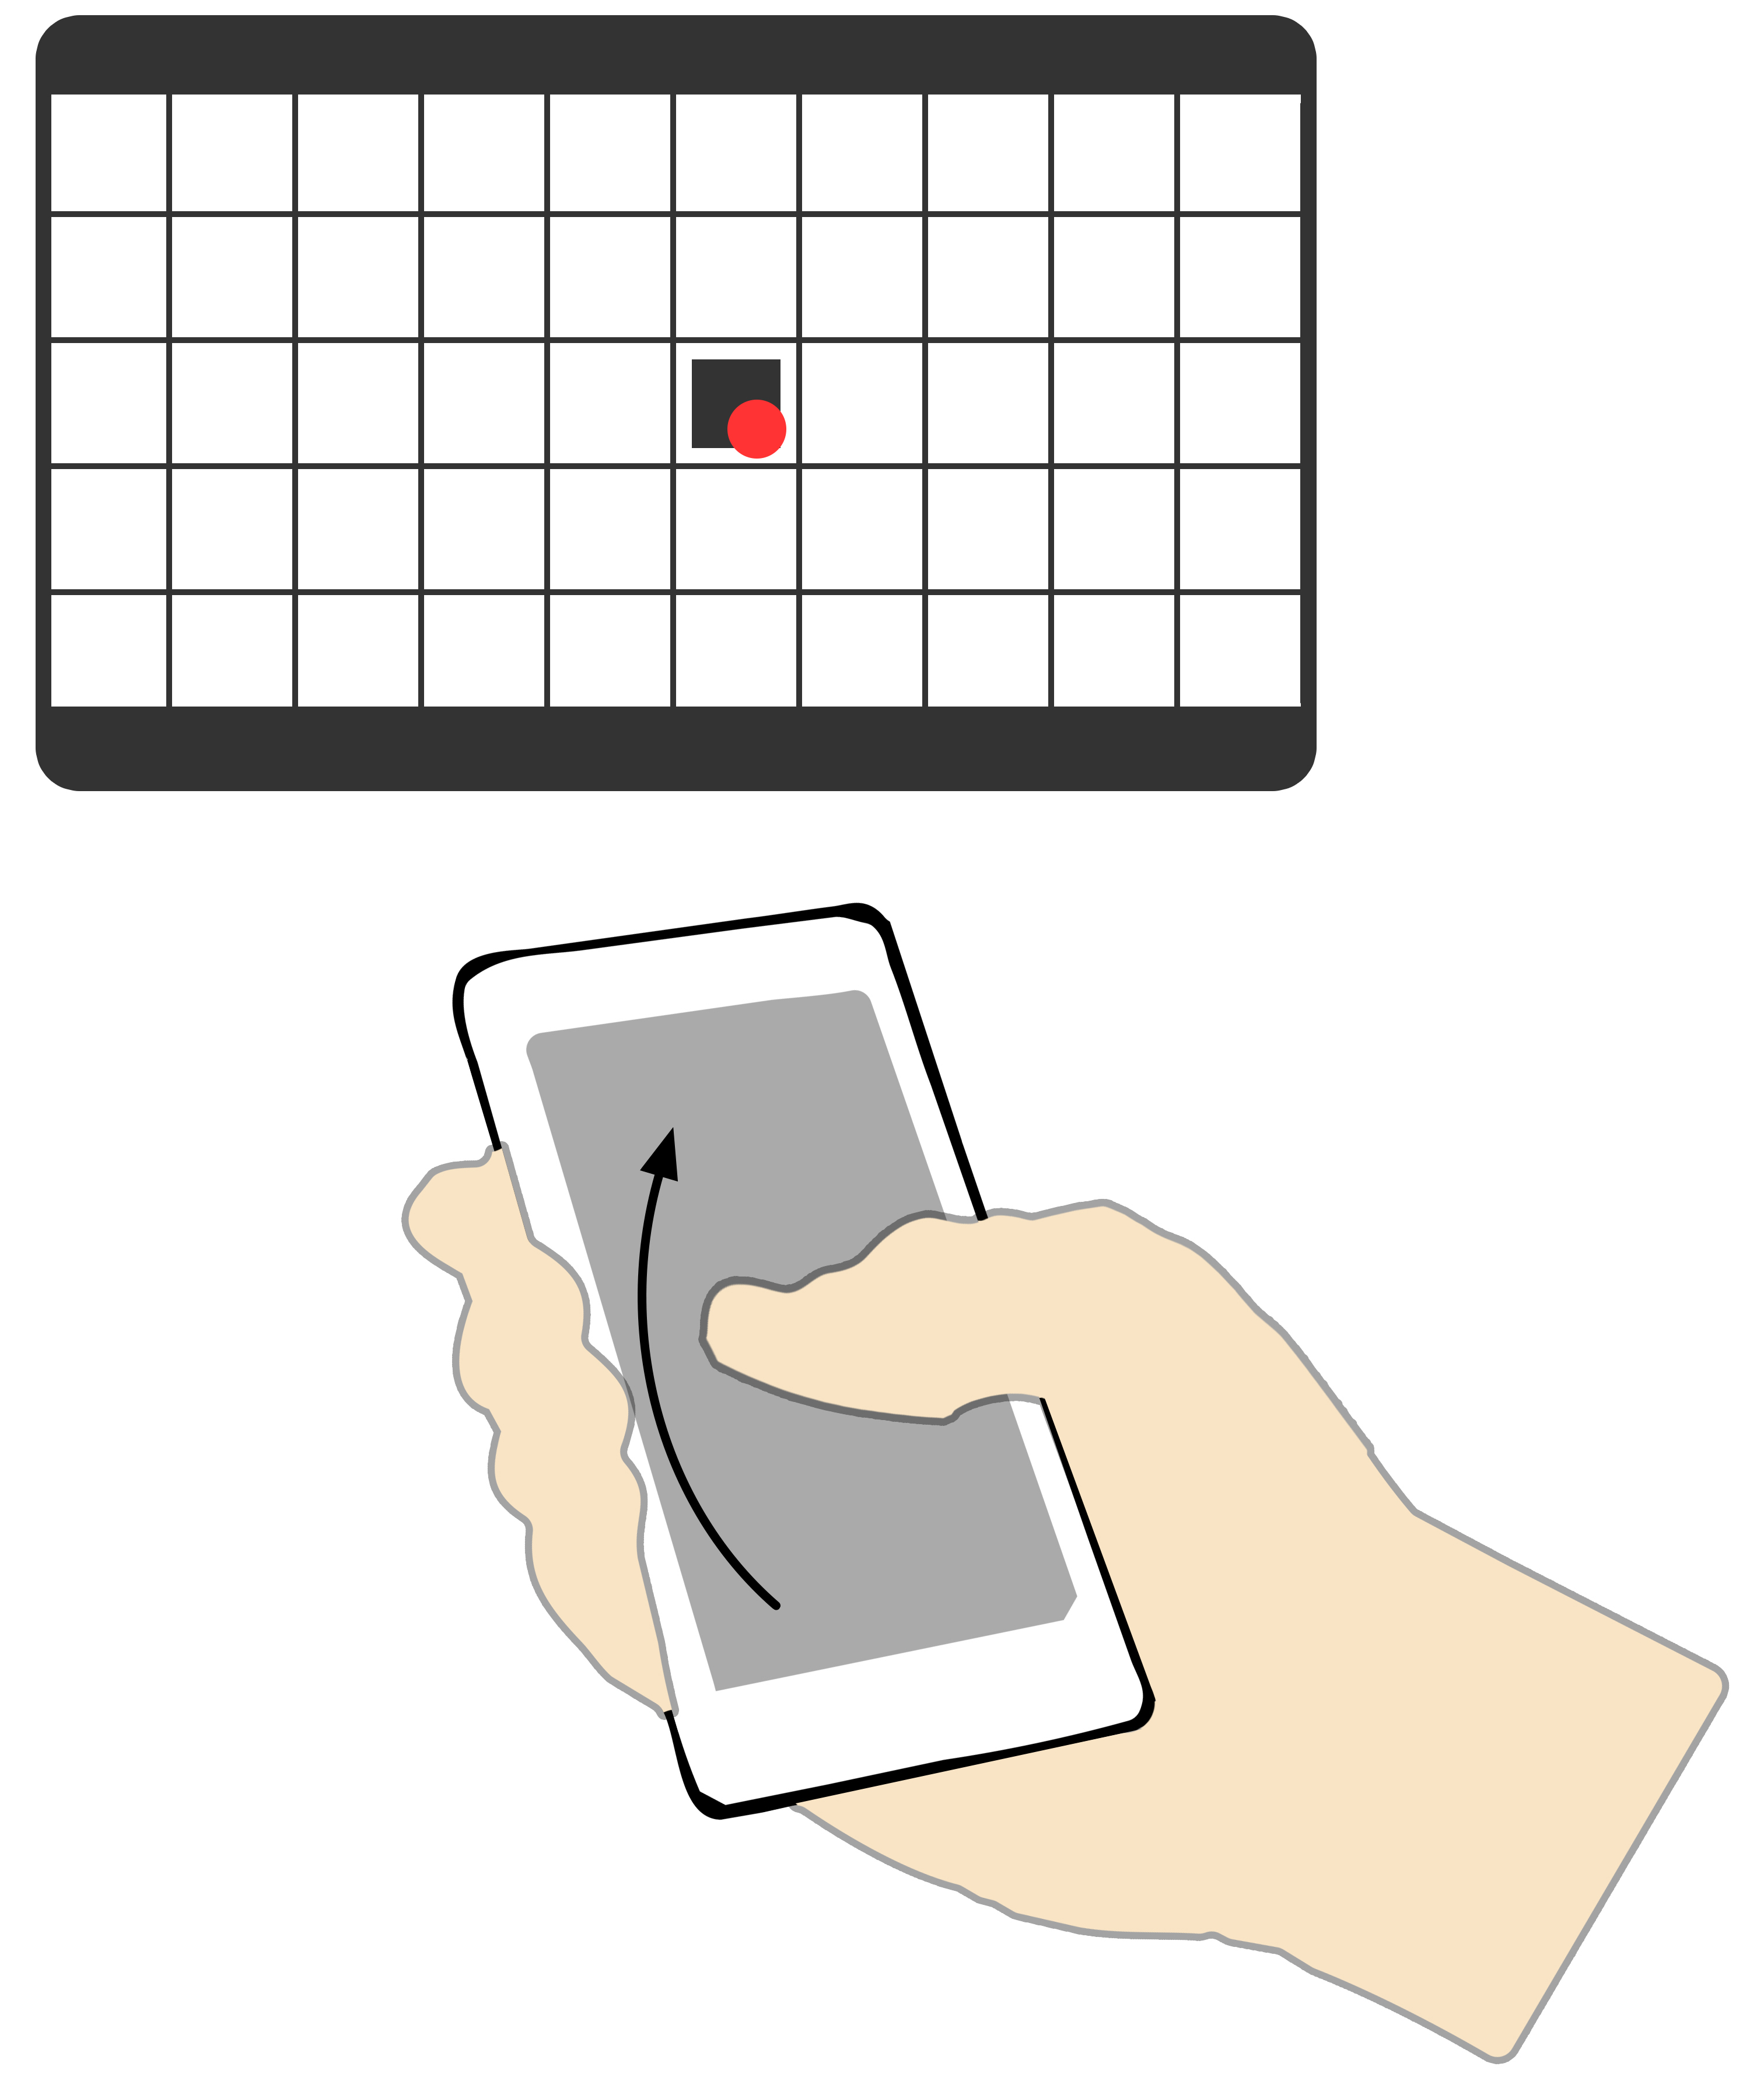
\includegraphics[width = 0.33\columnwidth]{images/swipe_b.jpg}\label{fig:swipeTechniqueB}}
	\subfloat[]{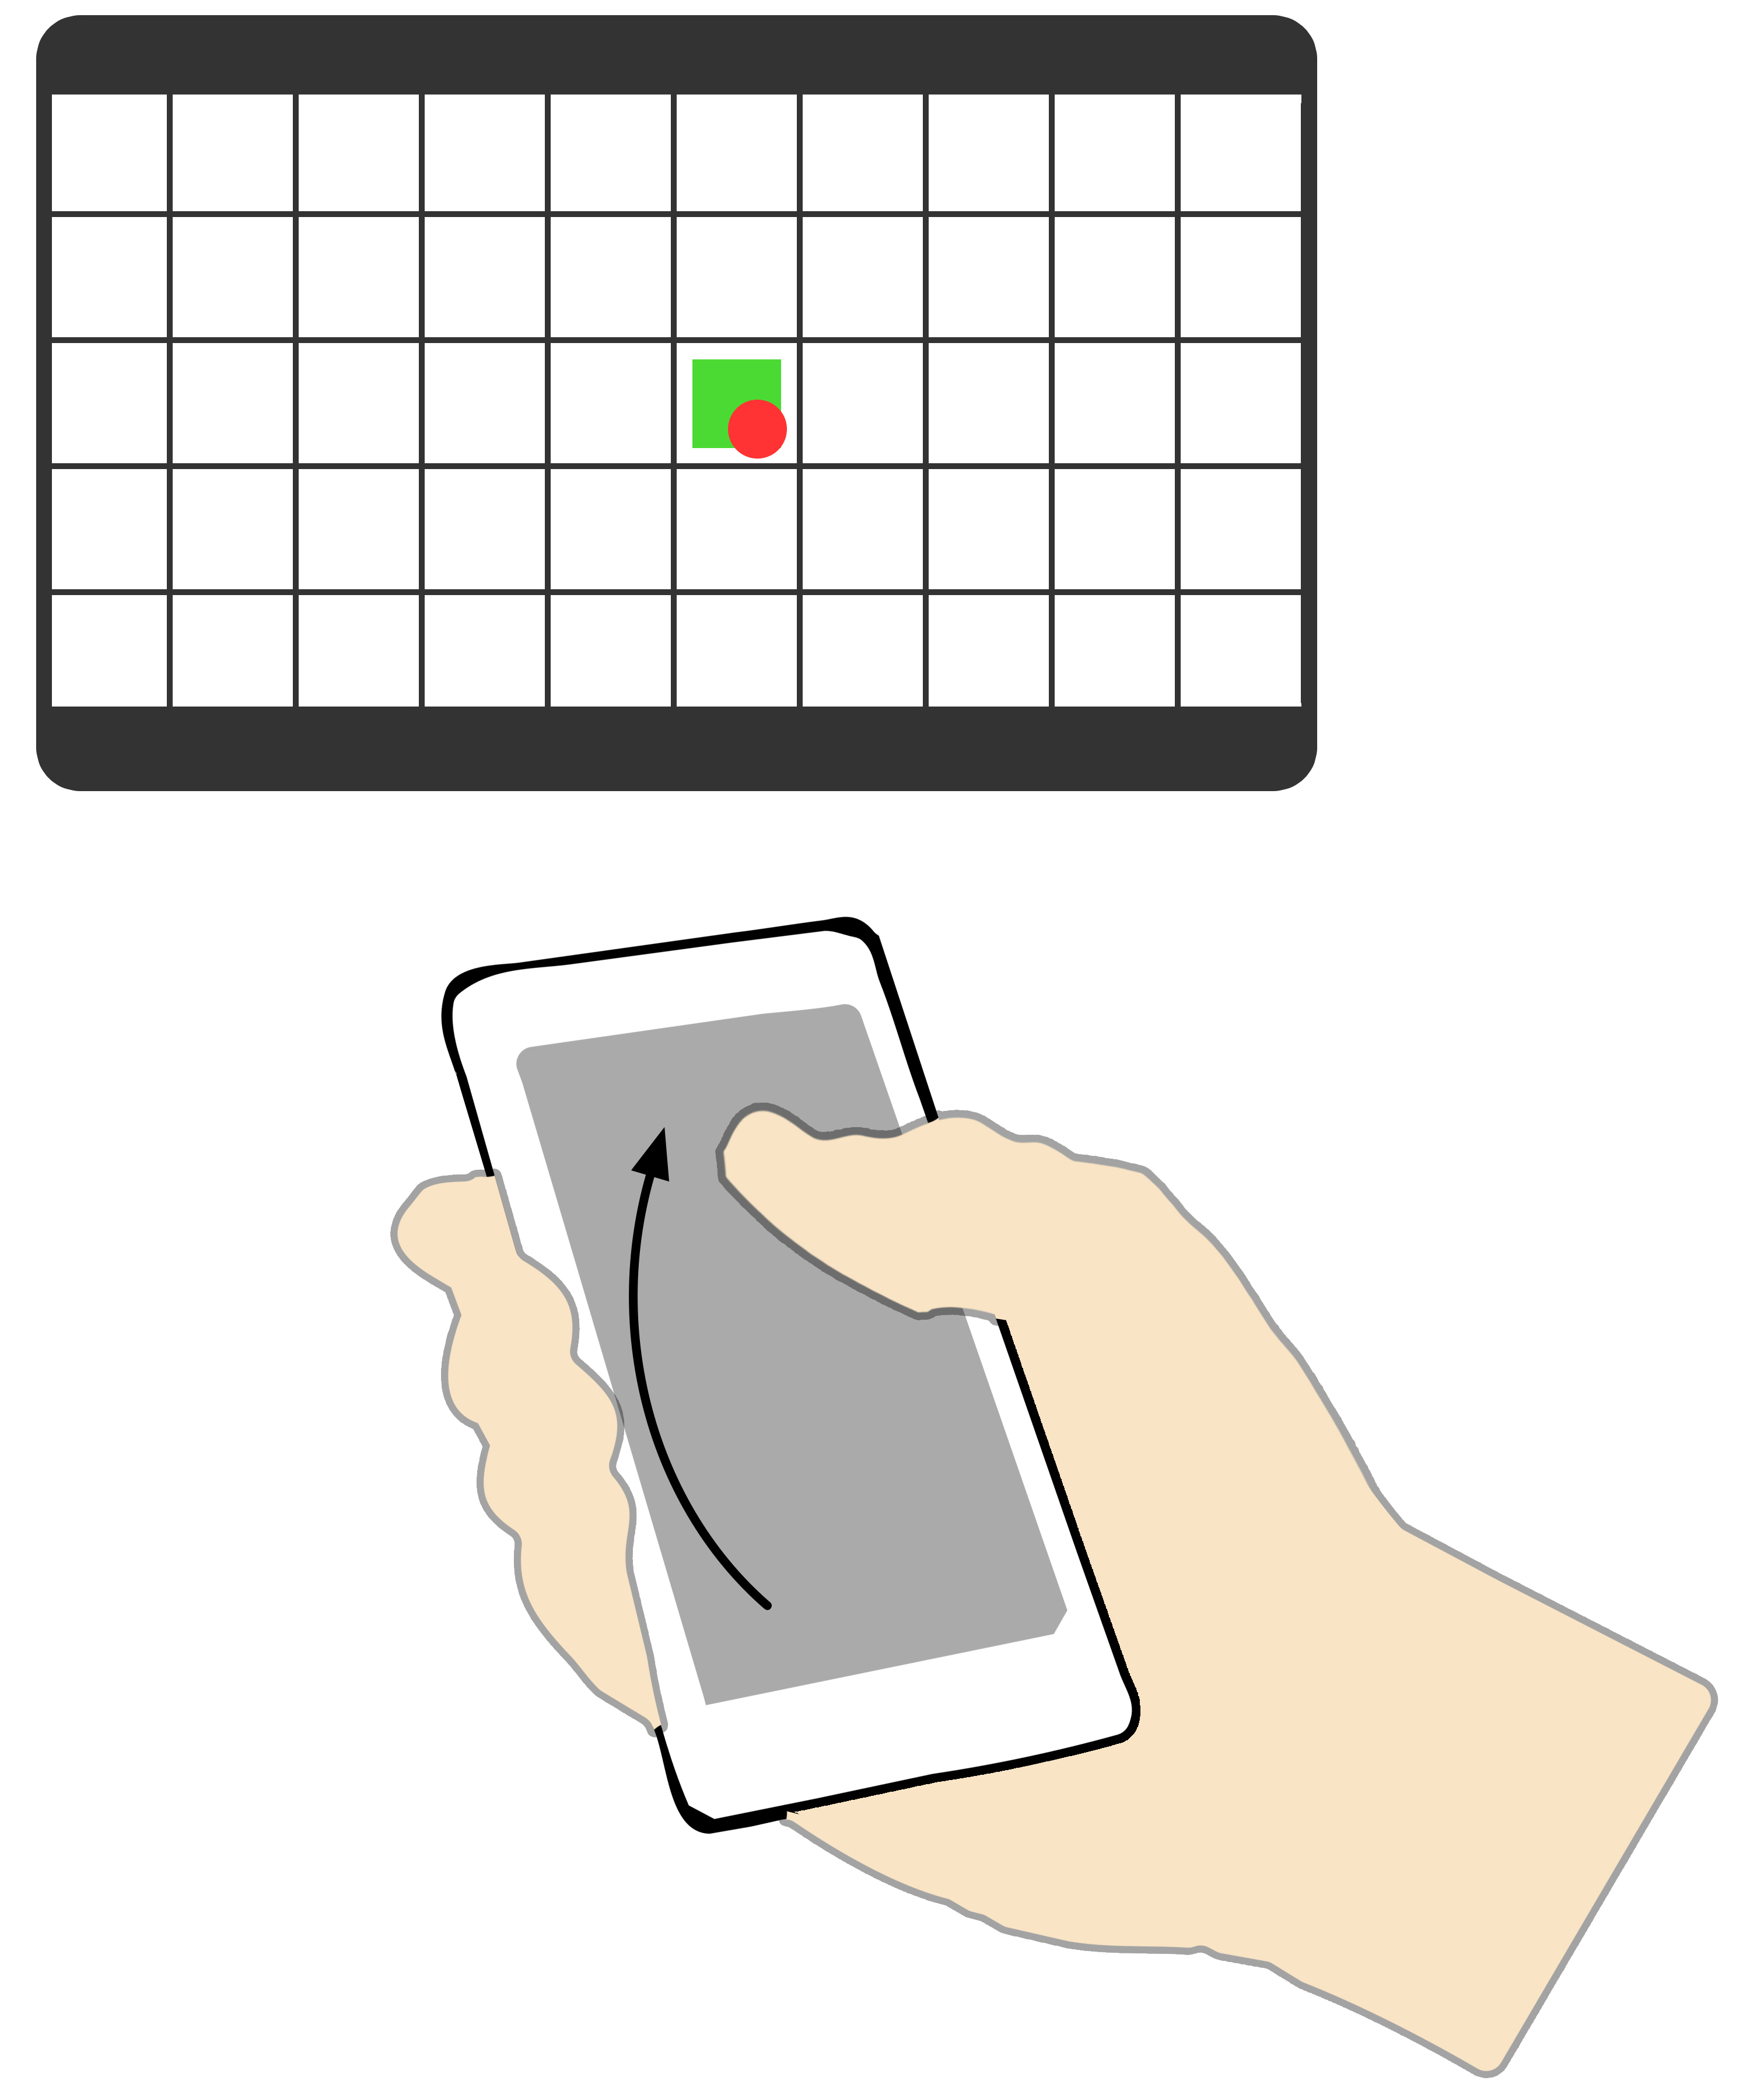
\includegraphics[width = 0.33\columnwidth]{images/swipe_c.jpg}\label{fig:swipeTechniqueC}}
	\label{fig:swipeTechnique}
\end{figure}
